\noindent\rule{3cm}{0.2pt}

\subsection{Blueprint}
\textit{
\begin{enumerate}
    \item Describe what models will be used
    \item Briefly describe what BERT is
    \item Mention that models without BERT will be compared with the ones with BERT
    \item Performance measures
    \item Dataset selection and preparation
    \item Steps made during the modeling
\end{enumerate}
}

\noindent\rule{3cm}{0.2pt}
\\

Access to high-quality data is a significant challenge faced in data modeling and machine learning. In the absence of high-quality data, it is impossible to construct accurate machine learning models. Poor quality data, characterized by unreliable data collection methods, a large number of errors, incompleteness, or mislabeling, can compromise the effectiveness of any machine learning algorithm. This issue is particularly pertinent in the context of datasets containing fake news, where labeling is not as straightforward as with other datasets. The task of manual labeling, which is required to obtain ready-made texts labeled as fake news or real information, can be both time-consuming and challenging, requiring substantial trust in the person performing the labeling. As such, the labeling process is prone to significant human error, which can impact the selection of an appropriate dataset.

This research article aims to investigate how the use of various natural language processing (NLP) methods influences the accuracy of fake news prediction, rather than building a model to accurately predict fake news. Therefore, when selecting a dataset, the most crucial considerations are the quality of the labeled observations and the consistency of the labeled texts across the entire dataset. Additionally, the text should closely align with the research area, as the focus of this study is on detecting fake news. To construct a universal tool for detecting fake news, the dataset should include varied topics and text characteristics, reflecting the real-world distribution as accurately as possible. In this way, the model can learn from natural data, picking up the nuances present in different texts, such as writing style, formality, and topics. However, as noted earlier, the primary objective of this article is not to construct a ready-made tool but rather to examine and impact the predictive quality of different NLP methods. 

The dataset chosen to carry out the research, which meets the criteria outlined above for a good dataset, is \href{https://www.kaggle.com/datasets/clmentbisaillon/fake-and-real-news-dataset}{\textit{Fake and real news dataset}}, obtained from the Kaggle website. The dataset comprises 40,000 observations, encompassing both authentic and fake news articles. Each observation is characterized by five variables that explicate the news item, namely, the news item's title, its content, the topic it pertains to, the date of publication, and a binary label denoting if the news is fake or not. Notably, the dataset is balanced, containing an equivalent number of true and fake news items.

The raw dataset underwent a process of data cleaning and feature engineering. The topics of the news articles were concatenated with their respective content, resulting in a longer text that retains all pertinent information. The cleaned texts were further processed by removing stopwords and punctuation marks. The topic information was omitted from the analysis as it unnecessarily complicates the dataset, potentially introduces uncertainty regarding its correctness, and is difficult to obtain for new data. Importantly, introducing additional variables would add noise to the prediction results, thereby complicating the analysis of the impact of different embedding methods on prediction accuracy. Similarly, the time variable of article publication was also omitted. The resulting dataset is now ready for further analysis and for applying embedding techniques to the news content.

\subsection{Embeddings (WIP)}
The next step after cleaning the data is to convert it in a way that is understandable to the computer. Textual data have the characteristic of forming a coherent whole. Individual letters form words, words form sentences, and sentences form longer pieces of text with a logical structure. Natural language is full of nuances. The same words can have different meanings and emotional connotations depending on the context. Understanding language comes naturally to humans and does not pose major difficulties. The human brain easily captures the appropriate context of words and their meaning, combining them into a logical and coherent text.

However, computers operate in a completely different way than the human brain. Computers are only capable of analyzing sequences of bits, which when arranged in a specific order, yield a result in the form of an element of a larger whole. This way, a sequence of bits can be presented as individual letters. Further, a sequence of letters can be represented as words. Then, in the tokenization process, individual words can be assigned a specific number. This way, the computer is able to decode the data represented by these words into something it can understand.

Nevertheless, the problem of conveying a deeper understanding of the text, the meaning of individual words, and the semantic relationships between them as understood in terms of similarity and analogies, still remains to be solved. The answer to this problem is Word Embedding. Word Embedding is used to represent words using numerical vectors, in such a way that the distance calculated between two words that are semantically similar is small, and between two semantically different words is large.

The Figure~\ref{embedding_example} illustrates the graphical interpretation of Word Embedding, often encountered in the literature. Similar words, such as King and Queen, Man and Woman, are closer to each other in the vector space. Two dimensions can be interpreted. The first dimension determines the fact of being a member of the family, while the second dimension indicates gender.

\begin{figure}[hbt!]
\centering
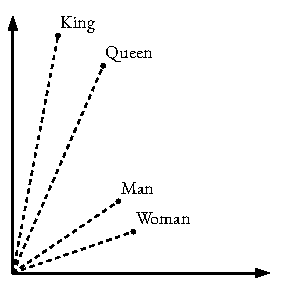
\includegraphics[width=0.75\linewidth]{embedding_example.pdf}
\caption{Smilar words are closer together}
\label{embedding_example}
\end{figure}

Trained unsupervised machine learning algorithms handle the conversion of words into vectors from large sets of textual data. These algorithms learn to predict the context of a given word by analyzing the words with which it is associated. In this process, they learn the context of words and the semantic relationships between them. Examples of such algorithms include BERT, Word2Vec, and GloVe.

\subsubsection{BERT}
\textit{Description of BERT embedding method...}

\subsubsection{GloVe}
\textit{Description of GloVe embedding method...}

\subsubsection{Word2Vec}
\textit{Description of Word2Vec embedding method...}


\subsection{Classification algorithms (WIP)}
\textit{Describe what classification algorithms has been used and what are the pros and cons for each of them...}

\subsubsection{K-nearest neighbors algorithm (KNN)}
\textit{Description of KNN algorithm...}

\subsubsection{XGBoost}
\textit{Description of XGB algorithm...}

\subsubsection{Random Forest}
\textit{Description of Random Forest algorithm...}

\subsubsection{SVM Classifier}
\textit{Description of SVM Classifier algorithm...}





\begin{figure*}
\centering
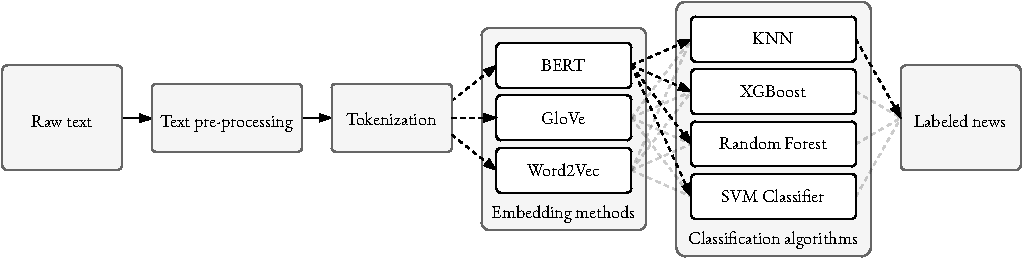
\includegraphics[width=0.8\linewidth]{methodology-schema_extended.pdf}
\caption{Architecture of each embedding-classifier model combination}
\label{methodology-schema_extended}
\end{figure*}


\subsection{Metrics (WIP)}
\textit{Description of used performance metrics..}

\subsection{Results (WIP)}

\begin{table}[hbt!]
\begin{threeparttable}
\caption{BERT Embeddings results}
\label{bert_embeddings_results}
\begin{tabular}{lll}
\toprule
\headrow Model & Accuracy & F1-Score\\
\midrule
KNN & 96.5 & 96.5\\ 
XGBoost & 95.0 & 95.0\\ 
Random Forest & 94.0 & 94.0\\ 
SVM Classifier & \textbf{98.5} & \textbf{98.5}\\ 
Logistic Regression & 98.0 & 98.0\\ 
\bottomrule
\end{tabular}
%\begin{tablenotes}[hang]
%\item[]Table note
%\item[a]First note
%\item[b]Another table note
%\end{tablenotes}
\end{threeparttable}
\end{table}

\begin{table}[hbt!]
\begin{threeparttable}
\caption{GloVe Embeddings results}
\label{glove_embeddings_results}
\begin{tabular}{lll}
\toprule
\headrow Model & Accuracy & F1-Score\\
\midrule
KNN & 89.5 & 89.4 \\ 
XGBoost & 92.5 & 92.5 \\ 
Random Forest & 87.5 & 87.4 \\ 
SVM Classifier & 94.0 & 93.9 \\ 
Logistic Regression & \textbf{94.5} & \textbf{94.4} \\ 
\bottomrule
\end{tabular}
%\begin{tablenotes}[hang]
%\item[]Table note
%\item[a]First note
%\item[b]Another table note
%\end{tablenotes}
\end{threeparttable}
\end{table}

\begin{table}[hbt!]
\begin{threeparttable}
\caption{Word2Vec Embeddings results}
\label{word2vec_embeddings_results}
\begin{tabular}{lll}
\toprule
\headrow Model & Accuracy & F1-Score\\
\midrule
KNN & 91.5 & 91.4 \\ 
XGBoost & 96.0 & 96.0 \\ 
Random Forest & 91.0 & 91.1 \\ 
SVM Classifier & \textbf{97.0} & \textbf{96.9} \\ 
Logistic Regression & 95.5 & 95.4 \\ 
\bottomrule
\end{tabular}
%\begin{tablenotes}[hang]
%\item[]Table note
%\item[a]First note
%\item[b]Another table note
%\end{tablenotes}
\end{threeparttable}
\end{table}

\begin{table}[hbt!]
\begin{threeparttable}
\caption{KNN results}
\label{knn_results}
\begin{tabular}{lll}
\toprule
\headrow Embedding Method & Accuracy & F1-Score\\
\midrule
BERT & \textbf{96.5} & \textbf{96.5} \\ 
GloVe & 89.5 & 89.4 \\ 
Word2Vec & 91.5 & 91.4 \\ 
\bottomrule
\end{tabular}
%\begin{tablenotes}[hang]
%\item[]Table note
%\item[a]First note
%\item[b]Another table note
%\end{tablenotes}
\end{threeparttable}
\end{table}

\begin{table}[hbt!]
\begin{threeparttable}
\caption{XGBoost results}
\label{xgb_results}
\begin{tabular}{lll}
\toprule
\headrow Embedding Method & Accuracy & F1-Score\\
\midrule
BERT & 95.0 & 95.0 \\ 
GloVe & 92.5 & 92.5 \\ 
Word2Vec & \textbf{96.0} & \textbf{96.0} \\ 
\bottomrule
\end{tabular}
%\begin{tablenotes}[hang]
%\item[]Table note
%\item[a]First note
%\item[b]Another table note
%\end{tablenotes}
\end{threeparttable}
\end{table}

\begin{table}[hbt!]
\begin{threeparttable}
\caption{Random Forest results}
\label{rf_results}
\begin{tabular}{lll}
\toprule
\headrow Embedding Method & Accuracy & F1-Score\\
\midrule
BERT & \textbf{94.0} & \textbf{94.0} \\ 
GloVe & 87.5 & 87.4 \\ 
Word2Vec & 91.0 & 91.1 \\ 
\bottomrule
\end{tabular}
%\begin{tablenotes}[hang]
%\item[]Table note
%\item[a]First note
%\item[b]Another table note
%\end{tablenotes}
\end{threeparttable}
\end{table}

\begin{table}[hbt!]
\begin{threeparttable}
\caption{SVM Classifier results}
\label{svc_results}
\begin{tabular}{lll}
\toprule
\headrow Embedding Method & Accuracy & F1-Score\\
\midrule
BERT & \textbf{98.5} & \textbf{98.5} \\ 
GloVe & 94.0 & 93.9 \\ 
Word2Vec & 97.0 & 96.9 \\ 
\bottomrule
\end{tabular}
%\begin{tablenotes}[hang]
%\item[]Table note
%\item[a]First note
%\item[b]Another table note
%\end{tablenotes}
\end{threeparttable}
\end{table}

\begin{table}[hbt!]
\begin{threeparttable}
\caption{Logistic Regression results}
\label{lr_results}
\begin{tabular}{lll}
\toprule
\headrow Embedding Method & Accuracy & F1-Score\\
\midrule
BERT & \textbf{98.0} & \textbf{98.0} \\ 
GloVe & 94.5 & 94.4 \\ 
Word2Vec & 95.5 & 95.4 \\ 
\bottomrule
\end{tabular}
%\begin{tablenotes}[hang]
%\item[]Table note
%\item[a]First note
%\item[b]Another table note
%\end{tablenotes}
\end{threeparttable}
\end{table}